Durch das Vorgehen nach Abbildung \ref{tikz:abbKodierungUndDekodierung} und die beschriebenen Kodiermöglichkeiten kann die Zuordnung der Kamerapunkte und der Bildschirmpunkte erfolgen.
Mithilfe weiterer Schritte kann man daraus die Oberfläche rekonstruieren.
%
\begin{figure}[H]
	\centering
	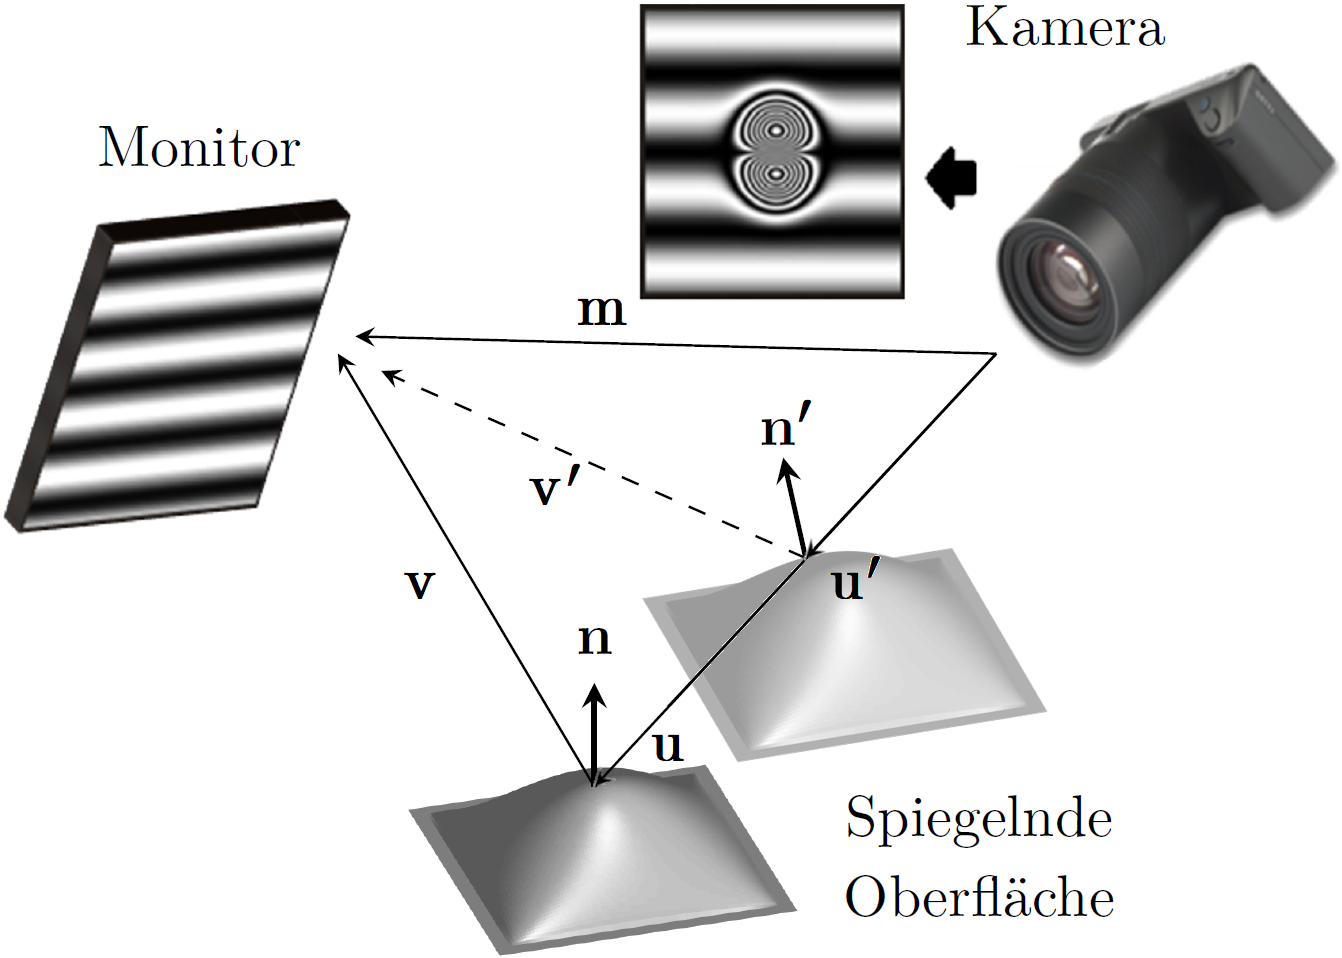
\includegraphics[width=0.7\textwidth]{02_grundlagenZurDeflektometrie/rekonstruktion/rekonstruktionUndRegularisierungsproblem/figures/regularisierungsproblem}
	\caption[Regularisierungsproblem]{Mehrere Positionsmöglichkeiten für die spiegelnde Oberfläche bei selber Zuordnung von Kamera- und Bildschirmpunkten, auch Regularisierungsproblem genannt. \textit{in Anlehnung an} \cite{stereoDeflektometrie}}
	\label{img:regularisierungsproblem}
\end{figure}
%
\noindent
Abbildung \ref{img:regularisierungsproblem} zeigt die Strahlenverfolgung zur Bestimmung der Oberflächennormalen $n$.
Zunächst benötigt man neben der Zuordnung zusätzliche Informationen über den Systemaufbau.
Das umfasst die Positionen und Ausrichtungen der Kamera und des Monitors im Raum, womit man die Zuordnung in Weltkoordinaten angeben kann.
Dadurch ist der Vektor $m$, sowie die Richtung des Sichtvektors $u$ bestimmt.
Man weiß zwar welcher Kamerapunkt welchen Punkt des Bildschirms sieht, allerdings ist dadurch das optische System nicht ausreichend beschrieben um die Länge des Sichtvektors $u$ anzugeben.
Es fehlt die Lage der Oberfläche.
Wäre diese bekannt, könnte der Reflexionsvektor $v$ mit 
\begin{equation*}
	v = m - u
\end{equation*}
bestimmt werden.
Mithilfe des Reflexionsgesetzes kann man aus dem Reflexionsvektor $v$ und dem Sichtvektor $u$ den Normalenvektor $n$ bestimmen:
%
\begin{equation}
	n = \dfrac{v - u}{\left\Vert v - u \right\Vert}
\end{equation}
%
Der Sichtvektor $u$ lässt sich für jeden Kamerapunkt aufstellen.
Berechnet man nach der Überlegung die Normalenvektoren $n$ für jeden Kamerapunkt, erhält man ein Vektorfeld, welches Normalenfeld genannt wird.
Damit wären die Neigungsinformation der Oberfläche bekannt.

\p
Durch die unzureichende Information über die Lage der spiegelnden Oberfläche, erhält man entlang der Richtung eines Sichtvektors $u$ unendlich viele potentielle Normalenvektoren $n'$.
Man bekommt somit auch viele verschiedene Normalenfelder für eine eindeutige Zuordnung von Kamera- und Bildschirmpunkten.
Diese Mehrdeutigkeit wird als Regularisierungs- oder Deflektometrieproblem bezeichnet \cite{regularisierungsproblem}.
Zur Auflösung des Regularisierungsproblems gibt es verschiedene Ansätze.
Ein solcher Ansatz ist die Stereo-Methode.
Dabei werden zwei Aufnahmen aus unterschiedlichen Positionen verwendet.
Man bestimmt für beide Aufnahmen jeweils eine Zuordnung von Kamera- und Bildschirmpunkten.
Somit entstehen für beiden Aufnahmen mehrere potentielle Normalenfelder.
Bestimmt man die Korrelation zwischen den Normalenfeldern der unterschiedlichen Aufnahmen, sollte man eine Lage finden, an denen die Normalenfelder übereinstimmen.
Das Normalenfeld in dieser Lage entspricht damit dem tatsächlichen Normalenfeld (siehe Abbildung \ref{img:stereoVerfahren}).
Dieses und auch andere Verfahren zur Auflösung des Regularisierungsproblems ist Thema der Dissertation von J. Balzer \cite{regularisierungsproblem}.
%
\begin{figure}[H]
	\centering
	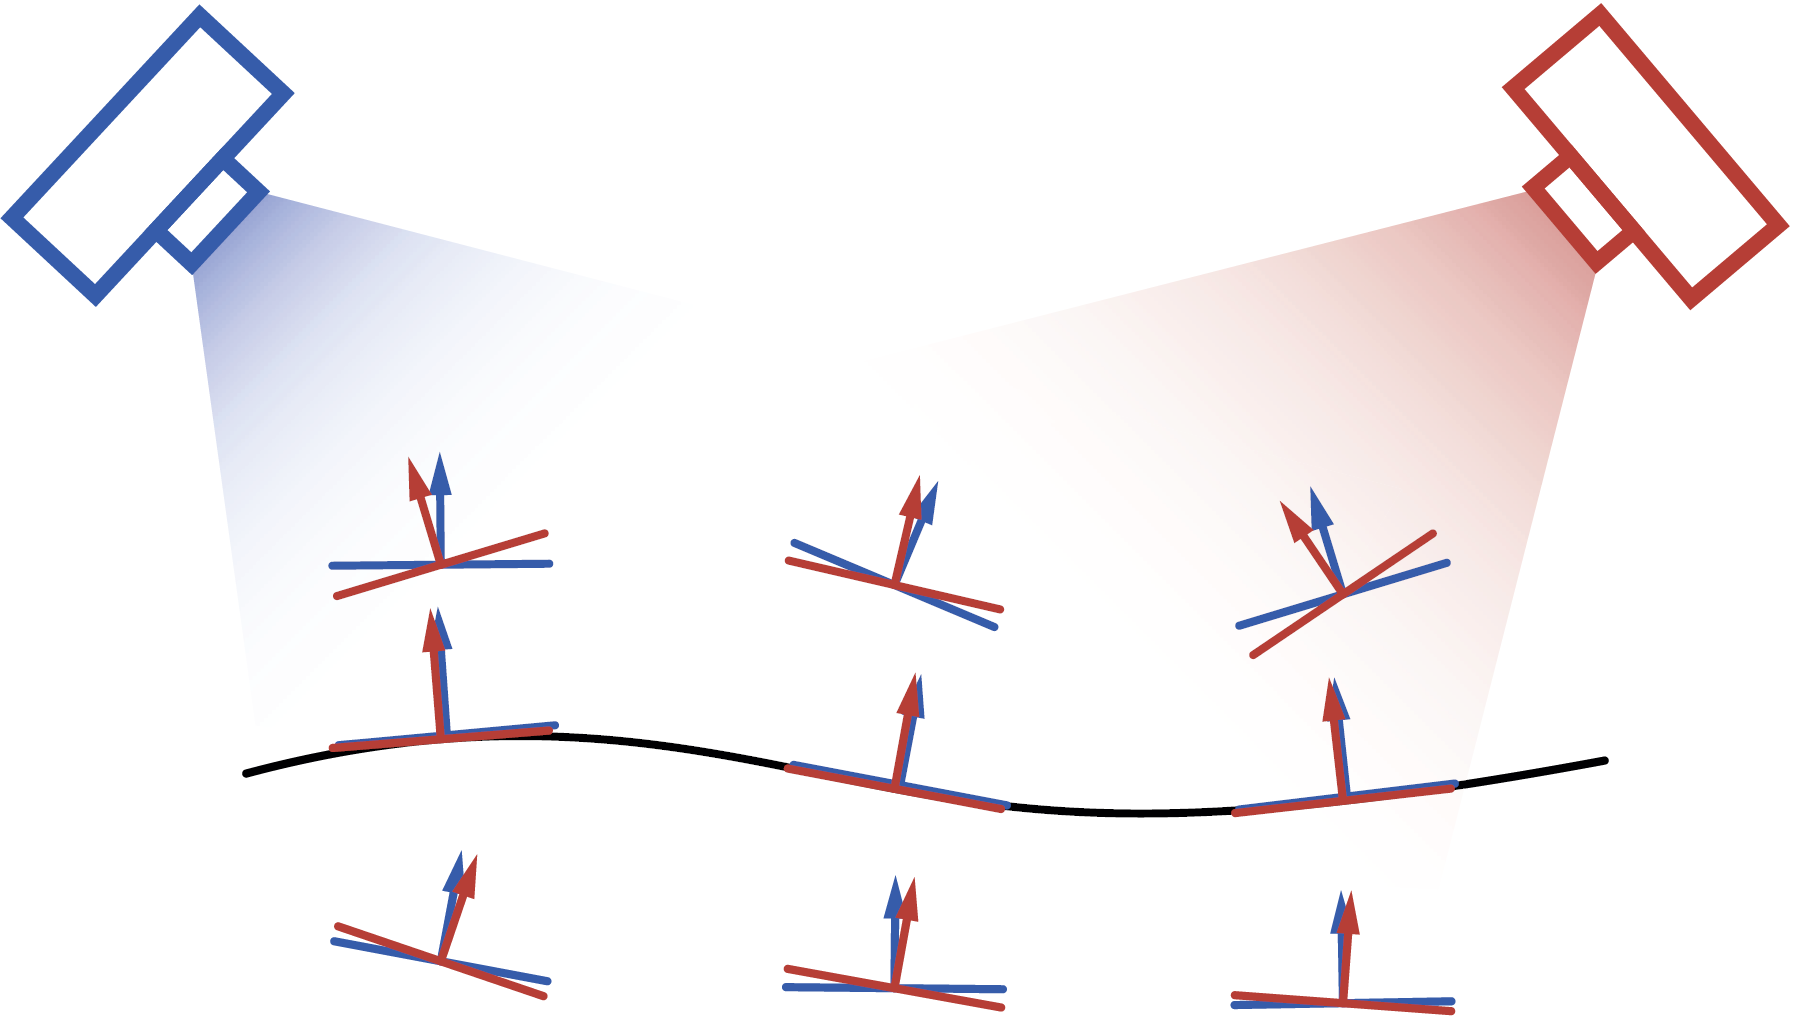
\includegraphics[width=0.5\textwidth]{02_grundlagenZurDeflektometrie/rekonstruktion/rekonstruktionUndRegularisierungsproblem/figures/stereoVerfahren}
	\caption[Stereo-Methode zur Lösung des Regularisierungsproblems]{Stereo-Methode zur Auflösung der Mehrdeutigkeit der Normalenfelder. Die eingezeichneten Pfeile sind die potentiellen Normalenvektoren auf unterschiedlichen Höhen. \cite{stereoDeflektometrie}}
	\label{img:stereoVerfahren}
\end{figure}
%
\noindent
Schließlich ist es möglich, aus dem Normalenfeld die räumlichen Informationen der Oberfläche zu berechnen.
Dafür kann man zunächst aus den Normalenvektoren die zugehörigen Tangentialebenen berechnen, die über je zwei Richtungsvektoren definiert sind.
Diese Richtungsvektoren bilden die Tangentialfelder des Prüfobjekts.
Man kann über eine Integration der Tangentialfelder in ausgewählte Richtungen Kurven bestimmen, die in der Oberfläche des Objekts liegen.
Durch diese Integration erhält man einen Höhenzusammen\-hang der Oberflächenpunkte.
Wenn zusätzlich die Lage eines Oberflächenpunkts im Raum gegeben ist, kann man die Positionen der Oberflächenpunkte im Raum angeben \cite{kit_werling}.